\documentclass[12pt]{report}
\usepackage{blindtext}
\usepackage{hyperref}
\usepackage{tocloft}
\usepackage{natbib}
\usepackage{graphicx}
\usepackage[newfloat]{minted}
\usepackage{caption}
\usepackage{booktabs}
\usepackage[toc, page]{appendix}
\usepackage{multirow}
\usepackage{subcaption}
\usepackage[margin=0.8in]{geometry}
\usepackage{csvsimple}
\usepackage{longtable}
\usepackage{array}
\setcounter{tocdepth}{3}
\setcounter{secnumdepth}{3}
\newenvironment{longlisting}{\captionsetup{type=listing}}{}
\newenvironment{code}{\captionsetup{type=listing}}{}
\SetupFloatingEnvironment{listing}{name=Code}
\makeatletter
\def\blfootnote{\xdef\@thefnmark{}\@footnotetext}
\makeatother

\title{%
  GPT-2 Based Story Teller\\
  \large CTEC3451 Development Project \\~\\
    De Montfort University
  \blfootnote{Word count: 7998}
} 
\author{Artem Bobrov (P2547788)}
\date{May 5 2022}
\setlength{\parindent}{1em}
\begin{document}
\maketitle
\thispagestyle{empty}
\clearpage
%TC:ignore
\section*{Abstract}
\addcontentsline{toc}{section}{Abstract}
\paragraph{}
The project described in this report is a story-telling application that uses the GPT-2 model to generate text. 
The model is trained on multiple datasets and is able to generate text from a variety of topics in the backend. 
The frontend is a web application that allows users to endlessly generate stories accompanied by thematic pictures.
The point of the project is to prove the concept that neural networks, if trained properly, are able to generate 
data that is very similar to human language.
%TC:endignore
\tableofcontents
\setcounter{tocdepth}{1}
\thispagestyle{empty}
\clearpage

\section*{Introduction}
\addcontentsline{toc}{section}{Introduction}
\paragraph{}
Neural networks weren't so popular in the early days of computing, but they are now a common tool for machine learning.
First neural network was invented by Frank Rosenblatt in the late 1950s \citep{rosenblatt_1958_the}. Perceptron has only 
one layer of neurons, but more advance neural networks can have multiple layers. Before Transformer neural networks 
there were many different types of neural networks (e.g. Convolutional, Recurrent, LSTM, Feed Forward, etc).

Transformers were introduced in 2017 by Google \citep{attention_is_all_you_need} and are a new type of neural network. It uses self-attention mechanism 
to focus on the most relevant information in the input. It weights the significance of each part of the input differently.

This report focuses on the GPT-2 model, which is a transformer type neural network developed by OpenAI in 2019 \citep{radford_wu_child_luan_amodei_sutskever_2019}.
Despite the fact that GPT-3 is a newer model, it's predecessor is still a popular choice for text generation.

An application will be developed that utilises the features of GPT-2 and wraps it up in a user-friendly web
interface that allows users to read freshly generated stories accompanied by thematic pictures. The development process 
will be examined and the results will be presented and discussed in depth. The usage of the key elements and techniques used both in
backend and frontend will be explained. Moreover the project development and research cycle will be reflected on and 
other approaches that possibly could have been used to achieve different or similar results will be presented.

\section*{Objectives and Goals}
\addcontentsline{toc}{section}{Objectives and Goals}

\subsection*{Initial approach}
\addcontentsline{toc}{subsection}{Initial approach}
\paragraph{}
It is important to state that the original plan for the project was to develop a similar application that generates
pictures with attached text to them (known as `memes') and allows users to watch them using a web interface. It has been
planned to use different approach to build a repository of training data using `Optical Character Recognition (OCR)' \citep{tesseract_article} and 
`Pillow' library to attach processed text to the pictures. It has been decided to adjust the original plan and change the
topic from memes to stories.

\subsection*{New approach}
\addcontentsline{toc}{subsection}{New approach}
\paragraph{}
The new approach doesn't require any massive changes to the original plan and the project will be developed using the same
techniques - indetical frontend and almost the same backend. The only difference is that OCR will be removed from the backend
because it's not needed for the project anymore. To minimize the deviation from the original plan, there will be an
additional section in the web interface that creates `memes' based on novels and other piece of art.

\clearpage

\subsection*{Reasons}
\addcontentsline{toc}{subsection}{Reasons}
\paragraph{}
Despite the fact that many of the features used in the initial approach have been already developed - Tesseract OCR, 
Pillow Image placing, `Meme' scraper - one major issue made it extremely perplexing to continue the project without changing the approach.

The first puzzling part was hidden in reading the text (using Tesseract OCR) from the scraped images and translate them to text strings.
Memes contain text captions that makes it easy for a human to read, but this same process is hard for machines to do so - 
especially via OCR. There were some images successfully processed by it but it didn't satisfy the requirement because the the success rate was too low.
Many solutions were tried, but even pre-processing the images before feeding them to the OCR engine didn't seem to give much improvement.
The second complexity was to build a meme repository itself. Using the meme scraper is not the best solution because
the content obtained by it can be anything. Unfiltered, uncensored - it's a huge ethical problem.

\subsection*{General Description}
\addcontentsline{toc}{subsection}{General Description}
\paragraph{}
Two general components of the development project are described in two sections. Such apparent separation between these categories 
is due to the fact that this approach allows a simpler, faster and more effiecient implementation with better user
experience, it also improves code readability and maintainability.

The first one is the backend, which is responsible for generating text based on given datasets 
(stories, novels, other pieces of art, etc). It is implemented in Python and uses numerous libraries
to achieve the goal. Multiple steps are involved in generating simple text samples including hours of training.

The second component is the frontend, which is a web application that creates a user-friendly, simple interface
to scroll and read stories. It is implemented in JavaScript using many libraries, as well as the Python part.
Such approach to frontend was chosen because web development is flexible and it's easy to adapt to different
platforms. Also it's possible to extend it to a web service that doesn't require downloading the application
to user's computer.

The goal is create a system with pre-trained model, which the user can use to scroll through the stories and 
react to each story leaving a positive or a negative feedback - using the `Like' and `Dislike' buttons. Afterwards,
these reactions will be stored in a database to be used by the developer to understand which stories should be
corrected and improved. The feedback system is designed to create a reflection on the pre-trained model as a whole and
not on separate elements (stories). Given the feedback, the developer can decide to improve the model or not.

\clearpage

\section*{Major Components}
\addcontentsline{toc}{section}{Major Components}

\subsection*{Backend}
\addcontentsline{toc}{subsection}{Backend}
\paragraph{}
% General info - Python, PyCharm
The backend of the project is developed using Python programming language since it's a very popular language for machine learning
and has a lot of libraries that can be used to achieve the goal. The backend is developed using PyCharm IDE, which is also
a popular editor for Python. Calculations that are done in the backend can be executed on any machine with Python 
installed. The only issue is the optimisation - text generation requires a lot of computing power.

\subsubsection*{GPT-2 and the library}
\addcontentsline{toc}{subsubsection}{GPT-2 and the library}
\paragraph{}
% Libraries used to operate with the model
GPT-2 is the version of the GPT family used in the project. To operate with the network it was chosen to use a 
library called `GPT-2-simple' \citep{gpt-2-simple-git} since it features an easy approach to control and train the model.
The library is written in Python and offers a documentation which was used in order to work with the neural network.
GPT-2-simple offers two types of models - one with 124 million parameters and one with 324 million parameters. 
Acknowledging the computational limits of the processing unit used - graphical (GPU), the first model with 124 million
parameters was used. It is possible to use the second model but it requires a GPU with significantly more processing power and
memory. 

It is possible to use techniques that allow to save memory and train bigger models using memory saving gradients -
the main memory loss in the computation is due to calculating the gradient of the loss by backpropagation. At the
cost of one additional forward pass, the memory consumption can be reduced significantly \citep{chen_2016_training}.
However Tensorflow framework (version 2), which is used by GPT-2-simple, is not optimized for such tasks.

Despite providing simpler control functions, this library also provides a lot of tweaking options. For example, 
some of the hyperparameters can be changed to improve the model performance during testing. Learning rate, batch size,
number of training steps, number of accumulated gradients and optimizer can be changed. Number of layers and other
more complex parameters can also be changed but in order to do that, the parameters must be examined and adjusted in Tensorflow
code files.

The library also provides a way to load the model from a checkpoint file. This is useful when the model is trained
in multiple steps and it's needed to continue training from the last checkpoint without losing progress.

Another important feature for testing and optimising the output is the possibility to use different optimisers.
`Adam' and `SGD' are available optimisers. The first one is the most popular and is used in the project because 
the learning time is relatively short and the memory requirements are little \citep{musstafa_2022_optimizers}. 
These two aspects are crucial and thereforce the choice fell on `Adam'.

% Checkpoints, hyperparameters, adam


\subsubsection*{Datasets}
\addcontentsline{toc}{subsubsection}{Datasets}
\paragraph{}
% Alice, Catcher, Iliad, main problem - too much text decoration
% Iliad was formatted - removed all book names and multiple dashes
Several datasets are used in the project. It has been chosen to use three datasets to work with. The first one is
the novel `Alice in Wonderland' by Lewis Carroll \citep{alice_in_wonderland}. This version was taken from GitHub Gist.
It's more adapted for machine learning than the original version since it's shorter and therefore contains less tokens.
For the reason that it was the first dataset to train the network on, it has been decided to go with the shortened version.
The text file with the novel poses a certain inconvenience because it contains a lot of text decoration which can create
noise in the model. But also it can have a positive effect on the user experience because it can be perceived as a
unique style of the author. The unformatted version contains 26,413 words and 148,574 characters.

The second dataset used is the novel `Catcher in the Rye' by J. D. Salinger \citep{catcher_in_the_rye}. The version found on GitHub is
slightly incomplete in the beginning and therefore was filled with the original text from the book. Also it was slightly
formatted for the sake of the correctness of the output of the neural network. Chapter enumeration and the title page
were removed from the text file. In the final revision there are 73,676 words and 382,008 characters.

The last and the longest dataset is the novel `Iliad' by Homer \citep{the_iliad}. It contains 152,507 words and 807,481 characters.
It doesn't contain much text decoration apart from chapter (book) enumeration. Also it has some translation references and copyright information.
All this information was removed from the dataset since it could affect the training process. It still can be viewed in the original text document 
in the reference list. Another text decoration elements such as book (chapter) enumeration and dash symbols dividing the chapters was also removed.

Later as the project evolves more datasets potentially could be added. The main problem of having multiple datasets is the size of the
checkpoint files created by the neural network for training purposes. `Alice in Wonderland' checkpoint, which was trained 3,200 times on the novel
is around 500MB and `Catcher in the Rye' checkpoint is about the same size and the same amount of training steps. It would be possible to add more stories to the
project if the checkpoint storage would be located not on the user's machine but rather on a server.

\subsubsection*{Pillow}
\addcontentsline{toc}{subsubsection}{Pillow}
\paragraph{}
% Meme section
`Pillow' is a Python library used to manipulate images \citep{pillow_lib}. The reason why it was chosen to use in the development project is that it offers an easy and fast way
to insert text into the image. This process is also known as `meme' creation. It is possible to use generated samples
from the neural network, either cut the size of the samples after it has been generated or generate a small sample 
in the first place. The second option reduces the time of generation process but it also takes away the option
to format the text if the first and the last sentences are inappropriate. The customisation of the text in the library
is a very straightforward process. It is possible to change the font, the size, the colour, the position and the angle.

In terms of the project, `Pillow' will be used in the `Meme mode' section. The idea is similar to the stories generator,
the difference lies in the fact that the text is inserted into the image, rather than being printed below the image.
Stories are presented in a post-like format.


\subsection*{Frontend}
\addcontentsline{toc}{subsection}{Frontend}
\paragraph{}
% HTML, CSS, JavaScript
The frontend of the project consists of a mixture of HTML, CSS and JavaScript. HTML is a markup language which is used
to create the layout of the webpage. CSS is a language used to style the webpage. In this project it's used in a
bundle with Bootstrap for easier manipulations with the styles. JavaScript is used to control the behaviour of
the webpage and everything in it. Some of the functions displayed in the webpage are calculated and controlled 
solely with JavaScript with no interaction with Python.

\subsubsection*{Web Application appearence}
\addcontentsline{toc}{subsubsection}{Web Application appearence}
\paragraph{}
% Bootstrap, Electron, theme change
The application appearance is based on Bootstrap 5 and Electron. Bootstrap \citep{bootstrap} is a CSS framework/library 
that is used to create a responsive and mobile-first design. It's files (CSS and JS) can be accessed via `Content 
Delivery Links' (CDN). This method is useful when only a part of the content hosted on CDN servers is used in
development since CDN technology allows to deliver only necessary files. Also a big advantage is the loading time
if the resource is server-based by reducing latency \citep{cdnetworks}. The other aspect of the look is `Electron' which
was formerly known as `Atom Shell' \citep{a2015_atom}. It's a cross-platform application that is used to develop
application with web-like design. The main reason to work with `Electron' is the ability to have the same look and feel
on all platforms. GUI applications can be developed and deployed using web technologies much faster. Prior to the introduction 
of `Electron' to the project, the application was developed on the basis of different browsers and operating systems.

Also as can be seen on the figures below, most popular approach to the development of Python GUI apps - Tkinter, doesn't
satisfy the standards of app design in early 2020s. 

\begin{figure}[ht]
  \captionsetup[subfigure]{labelformat=empty}
  \centering
  \begin{subfigure}{.5\textwidth}
    \centering
    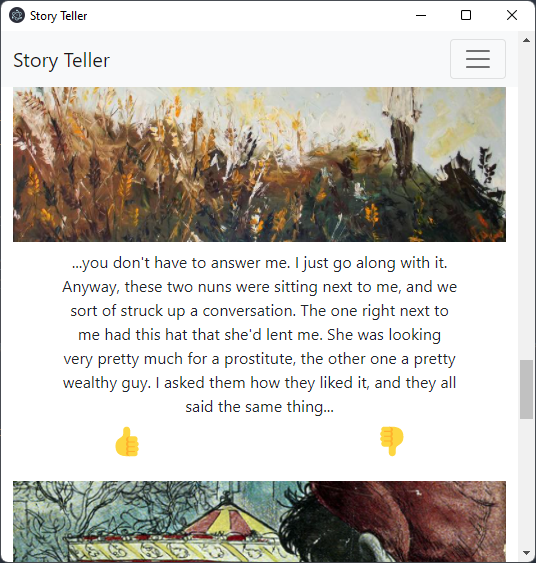
\includegraphics[width=.8\linewidth]{img/electron_window_example.png}
    \caption{Story Teller (Electron)}
    \label{fig:electron}
  \end{subfigure}%
  \begin{subfigure}{.5\textwidth}
    \centering
    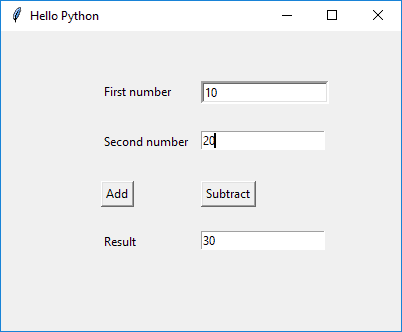
\includegraphics[width=.8\linewidth]{img/tkinter_window_example.png}
    \caption{Tkinter app}
    \label{fig:tkinter}
  \end{subfigure}
  \caption{A comparison of two GUI layouts}
  \label{fig:comparison_tk_electron}
\end{figure}

Similar situation occurs when it comes to animation with Tkinter. Many examples and many guides were examined and 
it has been concluded that Tkinter is not suitable for the purpose of the project because the aim of the project
is to create a fancy web-based application that can catch the attention of the user.

\clearpage

Another aspect of the design is the theme. Since many modern projects offer a possibility to change to 
either a light or a dark theme, it has been decided to develop an application with two themes. Bootstrap 
does most of the work for the theme change in terms of the colour change. Theme is persistent and is to a
settings file which is stored in the application's folder. On every start-up the application checks if the
theme is set to the light or dark mode accessing the JSON file.


\begin{figure}[ht]
  \captionsetup[subfigure]{labelformat=empty}
  \centering
  \begin{subfigure}{.5\textwidth}
    \centering
    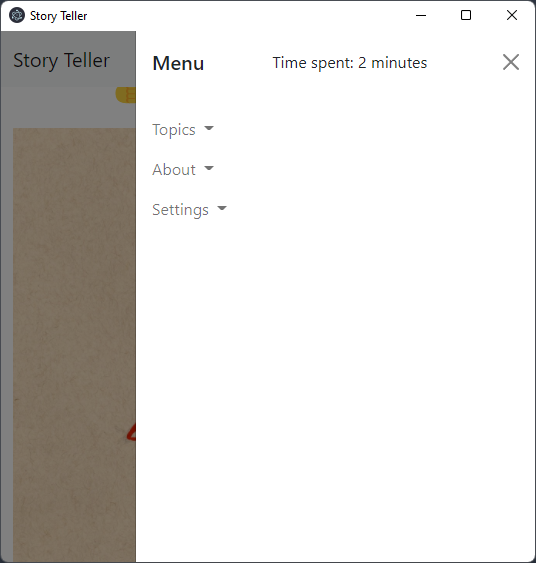
\includegraphics[width=.8\linewidth]{img/light_theme.png}
    \caption{Light theme}
    \label{fig:light_theme}
  \end{subfigure}%
  \begin{subfigure}{.5\textwidth}
    \centering
    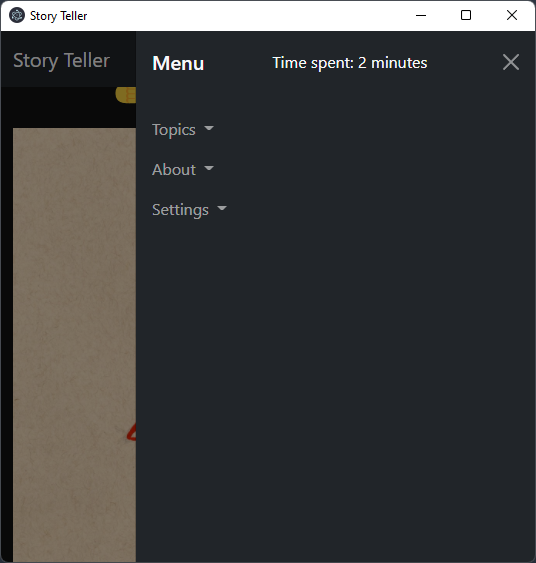
\includegraphics[width=.8\linewidth]{img/dark_theme.png}
    \caption{Dark theme}
    \label{fig:dark_theme}
  \end{subfigure}
  \caption{A comparison of two GUI themes}
  \label{fig:comparison_light_dark}
\end{figure}



\subsubsection*{Displaying the content}
\addcontentsline{toc}{subsubsection}{Displaying the content}
\paragraph{}
% Lazy loading, formatting the NN output, JQuery
To display the content it has been chosen to follow modern techniques of infinite scrolling. It loads
the content continously while the content is being generated on the fly. Infinite scrolling absolutely matches the 
topic of the project since the main idea was to create stories without any administrator intervention and 
minimise any unnecessary clicks and interactions. The content is displayed in a post-like format - that means 
a random picture from a set is followed by a random and freshly generated text based on a neural network checkpoint.
The displayed content depends on which topic is selected since the content is separated in different topics and 
displayed with different pictures.

Another aspect that needs to be considered is the conformity to accepted social standards.
In view of the fact that neural networks do not understand major human problems of inequality, supremacism and just
unacceptable language, a word filter can be used to filter out the most offensive words. That also might not be a problem
since the neural network generates text based on the source text fed into it.


\subsubsection*{User feedback}
\addcontentsline{toc}{subsubsection}{User feedback}
\paragraph{}
% Like and dislike buttons
User feedback is an easy and effective way to improve the application and enhance the text generation process in
particular. To establish a dialogue with a user the application uses a standard approach to the problem.
The user can either like or dislike the text generated by the application by simply clicking one of the buttons. 
It is planned to store the reactions in the database and use them to manually assess the quality of the content.
Comments are another possible solution to the user feedback problem but they seem too like a too complicated
approach.

\subsubsection*{Database}
\addcontentsline{toc}{subsubsection}{Database}
\paragraph{}
% Storing settings, user feedback, theme change, JSON
Databases are used to store the user settings and the user feedback. The settings are stored in a JSON file and are
accessed every time the application is started. JSON is a lightweight, human-readable text format that can be used with
any programming language. The objects in the files are stored in an `attribute-value' format. 

The purpose of the traditional database is defeated since the application doesn't store any sensitive information.
No encryption of the database is used either.

There are many other data serialisation formats such as XML, YAML, BSON etc. It has been decided to use JSON because
of its simplicity and flexibility compared to YAML. YAML is a superset of JSON and it seemed to big for the purpose.

%TC:ignore
\begin{code}
\begin{minted}[
frame=single,
framesep=3mm,
linenos=true,
xleftmargin=21pt,
tabsize=4]{js}
[
  {
    "Id": 0,
    "FirstName": "string",
    "LastName": "string",
    "Name": "string",
    "EmailAddress": "string",
    "TerritoryId": 0
  }
]
\end{minted}
\captionof*{listing}{An example of a JSON file}
\end{code}
%TC:endignore

\clearpage

\subsection*{Linking the frontend and backend}
\addcontentsline{toc}{subsection}{Linking the frontend and backend}
\paragraph{}
% Eel, Python, JavaScript
The main bridge between the frontend and backend used in this project is a `little Python library' 
called `Eel' \citep{knott_2022_eel}. It allows interaction between JavaScript and Python at every point of
the development. The library is used to create a web server that can be accessed from the browser - 
Chrome, Safari, Firefox and last but not least - Electron. 

The most important feature of `Eel' is function exposition. It allows to call any function that is explicitly 
defined with a `@eel.expose' decorator and use it anywhere in the JavaScript code and vice versa.

%TC:ignore
\begin{code}
\begin{minted}[
frame=single,
framesep=3mm,
linenos=true,
xleftmargin=21pt,
tabsize=4]{python}
@eel.expose
def count_files(path):
    return len(glob.glob1(path, "*.jpg"))
\end{minted}
\captionof*{listing}{Decorator for exposing functions}
\end{code}
%TC:endignore

\paragraph*{}
It's important to note that when a function call is made from the JavaScript code, it should be done in
async/await fashion. This is because the function call is made in the background and the result is returned
after some time.

The separation of the frontend and backend is an important action becasue it allowed to use the most efficient
approaches on each side and also focus on each part individually.

\begin{figure}[ht]
  \centering
  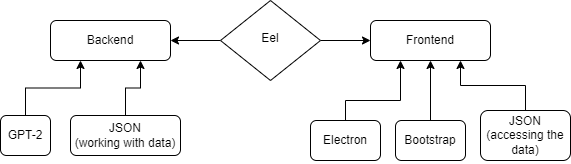
\includegraphics[width=1\linewidth]{img/system_diagram.png}
  \caption{The relations in the system}
  \label{fig:system_diagram}
\end{figure}

\clearpage

\section*{Development lifecycle}
\addcontentsline{toc}{section}{Development lifecycle}
\paragraph{}
Development process followed the principles of Agile practice. The main aspects of the development methodology
are: continiual improvement, flexible responses to any change and most importantly evolutionary development. Since
the project is developed by a single person, not a team, some of the practices of agile methodology are not applicable.

% Training sprint
% Implementation
% Testing
\subsection*{Training the model}
\addcontentsline{toc}{subsection}{Training the model}
\subsubsection*{Implementation}
\addcontentsline{toc}{subsubsection}{Implementation}
\paragraph{}
Training the model was a crucial step in the development process. Before the neural network would
be able to generate specific text based on some dataset, it has to be trained on it. The training process involves
tweaking many parameters of the model and the process is repeated until the best options are found. Currently,
all three checkpoints are trained with the same parameters and on the same model - 124M (124 million parameters). 
The finetuning process begins with a creation of a new session. Then the the finetuning function itself is called
with the following parameters: \textit{dataset name, model name, number of steps, name of the run, restore point,
overwrite option, length of the sample and an interval to save the checkpoints}.

Dataset name is the name of the preferred text file to train the network on. For this project three datasets were
chosen - Alice, Catcher and Iliad. Model name is the name of the model used in the training process. It can be either
`124M' or `355M'. The difference is in the parameter count. The `124M' model has 124 million parameters while the
`355M' model has 355 million parameters. Number of steps is the parameter that determines how many times will the
training process be repeated. For this project every checkpoint is trained more than 3,000 times in order to
produce a meaningful result. Run name parameter specifies which checkpoint is being trained. It is useful to have
multiple runs in the same model. Restore point and overwrite options are used for the sake of optimisation of the
process to minimise the chance of failing (crashing). Also the interval to save the checkpoints is set to a small
value of 100 to save the progress in case the process crashes.

%TC:ignore
\begin{code}
\begin{minted}[
frame=single,
framesep=3mm,
linenos=true,
xleftmargin=21pt,
tabsize=4]{python}
def train_model(self, run_name, file_name, steps, sample_length):
    sess = gpt2.start_tf_sess()
    gpt2.finetune(sess, file_name, model_name=self.model_name,
                  steps=steps, run_name=run_name, restore_from='latest',
                  overwrite=True, sample_length=sample_length,
                  save_every=100, sample_every=10000)
\end{minted}
\captionof*{listing}{Training function}
\end{code}
%TC:endignore

\clearpage

\subsubsection*{Testing}
\addcontentsline{toc}{subsubsection}{Testing}
\paragraph{}
\label{sec:model_testing}
Testing the training process is not a very long process itself, so it is not described in detail. The `GPT-2-Simple'
library offers many parameters to tweak and test the performance of the training process. All datasets were fed to the
network and trained on a machine with a `NVIDIA RTX 3080' GPU - this allowed an effective and speedy training process.

Several ways of training the neural network on the first dataset `Alice' were tried. The first attempt included
the raw format of `Alice in Wonderland' text file without any preprocessing (i.e. text is decorated with numerous
spaces, unnecessary punctuation marks and different symbols). The results from the training were acceptable and
the model was able to generate some of the samples that had sense in them. The second attempt included the preprocessing
of the original text file. Chapter enumeration, excess symbols and other punctuation was reduced in order to
minimise the impact on the network. Paragraph spaces were left in the text. The generated text was compared with the
original text and the results were satisfactory.

\begin{figure}[ht]
  \captionsetup[subfigure]{labelformat=empty}
  \centering
  \begin{subfigure}{.5\textwidth}
    \centering
    \fbox{
\includegraphics[width=0.9\linewidth]{img/alice-original.png}}
    \caption{Unprocessed text (trained 13,100 steps)}
    \label{fig:unprocess-alice}
  \end{subfigure}%
  \begin{subfigure}{.5\textwidth}
    \centering
    \fbox{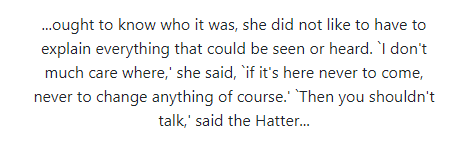
\includegraphics[width=0.8\linewidth]{img/alice-preprocess.png}}
    \caption{Prepocessed text (trained 1,000 steps)}
    \label{fig:preprocess-alice}
  \end{subfigure}
  \caption{A comparison of unprocessed and processed datasets}
  \label{fig:comparison_process_unprocess}
\end{figure}

The same process was applied to the second dataset `Catcher in the Rye'. It was cleaned from the chapter enumeration and
then fed to the neural network. It was trained more than 13,000 times.

The Iliad training was the fastest in terms of adjusting the text before feeding it. Since it didn't have any excessive
decoration and the paragraphs didn't have indents - the output text from the network was of a very good quality.

The finetuning parameters weren't tweaked much. The learning rate stayed at 0.0001 the gradient count was set to
5. As for the steps, it's impossible to identify a universal value for the best result. The best result for each
dataset was achieved by taking into account the accuracy of each training step. The longer and more complex the dataset -
the longer it takes to train. The final accuracy the neural network aimed to achieve was \textit{0.1-0.2}. Therefore
training times for every dataset are very different.

\subsubsection*{Reflection}
\addcontentsline{toc}{subsubsection}{Reflection}
\paragraph{}
Training the model was one of the most time-consuming parts of the project. Possibly, another method of training could
have been used. There's still a lot of freedom in what can be tweaked and changed in the parameter sections to
enhance the results of the training. For example, the biggest enhancement would be to use a different model with more
parameters. This project is limited computationally and therefore the model with the least parameters was chosen. The video
memory of the machine wasn't enough to train the model with 355 million parameters. There is a solution to that problem
as well (use memory saving gradients and only train transformer layers) but it's not implemented in Tensorflow 2.

\clearpage 

\subsection*{Text generation}
\addcontentsline{toc}{subsection}{Text generation}
\paragraph{}
Text generation sprint could have been placed together with model training sprint. However, it was decided to separate
the two because they are quite important on their own and whereas model training doesn't require frontend adaptation -
text generation does because it is the final product that is being presented to the user.
\subsubsection*{Implementation}
\addcontentsline{toc}{subsubsection}{Implementation}
\paragraph{}
Text generation is the most important part of the project. The function takes a trained checkpoint of the network and
based on the training it presents the user with a text. The function is written in a separate class based on the
`GPT-2-Simple' library. The function takes the following parameters: \textit{run\_name, length, nsamples}. These
parameters are thought to be the most `volatile' because they are changed often. The \textit{`run\_name'} parameter specifies
which checkpoint is being used. The \textit{`length'} parameter defines how many tokens the text should contain and the last parameter
\textit{`nsamples'} determines the number of samples to be generated.

% Exposed function for generating text
%TC:ignore
\begin{code}
\begin{minted}[
frame=single,
framesep=3mm,
linenos=true,
xleftmargin=21pt,
tabsize=4]{python}
@eel.expose
def generate_text(run_name, length, nsamples):
    sess = gpt2.start_tf_sess()
    gpt2.load_gpt2(sess, run_name=run_name, reuse=tf.compat.v1.AUTO_REUSE)
    texts = gpt2.generate(sess, return_as_list=True, length=length,
    nsamples=nsamples, model_name='124M')
\end{minted}
\captionof*{listing}{Exposed function for generating text}
\end{code}
%TC:endignore

\paragraph*{}
For the purpose of the infinite generation it is important to specify the \textit{`reuse'} parameter when the GPT-2
is being loaded. This parameter allows the model to be reused without the need to load it again. In the example above
this parameter is set to a value directly taken from the Tensorflow library since `GPT-2-Simple' provided explanation
in the documentation doesn't work (setting the `reuse' parameter to `True').

Yet this is only a first stage of the text processing in the function. After the text is generated it is handled by the
algorithm that is shown on the below figure.

%TC:ignore
\begin{code}
\begin{minted}[
frame=single,
framesep=3mm,
linenos=true,
xleftmargin=21pt,
tabsize=4]{python}
for idx, item in enumerate(texts):
    item = item.rsplit('.', 1)[0]
    if not item[0].isupper() and item[0].isalpha():
        item = '...' + item + '...'
    else:
        item = item + '...'
    texts[idx] = item
return texts
\end{minted}
\captionof*{listing}{Text processing algorithm}
\end{code}
%TC:endignore

The presented algorithm is developed specifically for this project. It is based on the idea that the text which is
output by the function is cut - it is been tested and proven in the previous section `Model training'. The incomplete
text seems to be cut only in the beginning and the end of the sample so, the algorithm iterates over the samples and
removes the last sentence from each of them. This is done using Python `rsplit' function which is the reverse version
of a standard `split'. After that, the first element of the word is checked for two conditions to decide where to put
the ellipsis. First condition - uppercase, second condition - alphabetic character. If this is the case, the ellipsis
is placed in the beginning and in the end of the word. If it's not - only in the end.

The point of the ellipsis is to make the text more pleasing to the eye and slightly confuse the perception of the user.
It's been decided to call this trick `Ellipsis of Uncertainty' - when the user sees the text that begins with 
ellipsis which signals that this is not the beginning of the text and ends with ellipsis which has the same meaning
in perception,e tex they won't expect to see a fully understandable piece of text.

\subsubsection*{Testing}
\addcontentsline{toc}{subsubsection}{Testing}
\paragraph{}
The testing process of the text generation involved the assessment of the generated text not only by the quality of
the output but also by how it looks displayed on the page appended to the image. It might seem that this testing
section overlaps with the testing section of the frontend development and it does, since the correlation between 
those elements is very high.

The main aspect of testing was the time taken to generate the text sample. It is important not to make the user
wait for too long because it may result in a loss of the user's attention. The \hyperref[appendix:model_testing]{model testing appendix}
shows different test cases and results of parameter tweaking. The most optimal parameters were found to be: length
of the text - \textit{100}, number of samples - \textit{6}. It satisfies the time requirement of 15 seconds for generating 
all 6 samples on whichever topic the user chooses. `Alice' checkpoint has been tested more than the other checkpoints due
to the fact that it's the first checkpoint that was developed. The results and knowledge gained from the testing are transferred
from `Alice' to other checkpoints successfully saving time.

\subsubsection*{Reflection}
\addcontentsline{toc}{subsubsection}{Reflection}
\paragraph{}
Output generation was a harder task to accomplish because it involved more than just using and adapting the functions
from the library but also a `Ellipsis of Uncertainty' trick had to be implemented. Also a lot of tests weren't passed
because the expected outcome was an uncut text. That case wasn't reached and thus the trick described above was used.
Besides, the text length was a question that had to be answered by testing what looks the best under a picture. 
Most likely, the reaction system will help to find out the best length and what exactly the user is looking for.
Generally assessing, the result might have been much better if the model with a higher number of parameters was used.
Having that said, it's hard to make a neural network that knows little words and sentences, generate a text that is
practically indistinguishable from the text that would come from a human. The benefit of having more parameters is that
the model can represent much more complicated functions that with fewer parameters.

\clearpage

\subsection*{Frontend Development}
\addcontentsline{toc}{subsection}{Frontend Development}
\paragraph{}
It has been decided to unify all the work carried out in the frontend into one section of the report. The reason for that
is a belief that the frontend must work as a one single unit since it consists of many small components that are unable to
work on their own. This section will include the implementation process of such elements as: navigation bar, menu,
content loading, reaction animations, theme change and other elements related to frontend (created and coded in the
JavaScript part of the project).

\subsubsection*{Implementation - Visible elements}
\addcontentsline{toc}{subsubsection}{Implementation - visible elements}
\paragraph{}
The implementation of the navigation bar was one of the first things that was done in the frontend. Bootstrap 5 was used
in order to create a responsive navigation bar. The navigation bar is a simple one with a hamburger menu button that leads
to a dropdown menu that contains the several sections to tweak the application. Instead of a logo on the left of the navigation
bar - application's name is displayed. Moreover, this name can be used as an active button to return to the beginning of the page.
That is a very useful feature in an infinite scrolling app.

A dropdown menu implements three sections. The first one is `Topics'. It contains three different sections that neural network
can generate text on. The second section is `About'. It contains information about the developer and a current version of the
application. The third section is `Settings'. A button to change the theme of the application is located there along with
mode selection. There are two modes of the app - classic and meme mode. In the classic mode the app generates text beneath
the images and the final content looks like posts. In meme mode the text is going to be appended directly onto the images to create
meme-like effect. Apart from the sections, the menu has a timer built into it. The timer counts how much time has passed since the
application was opened.

Post arrangement is designed following the main trends of the Internet nowadays. First comes the image then the description and
only after that are positioned the feedback buttons. The feedback buttons are animated when the user hovers on them. It's a simple
and effective way to show the user that the app is responsive and invites them to leave some feedback. If the desired reaction is clicked,
the button stays enlarged. All the content is dynamic on the page and is generated on the fly. Images are pulled from the array which is being
shuffled every iteration of post generation. 

Theme change implementation is heavily based on the Bootstrap 5. All of the elements use class togglers to change the theme.
Classes are implemented in Bootstrap and can be used on almost any element of the page. One of the complexities in the implementation
of the dark theme laid under the hood is the generating of the new posts with according colour of the text. When a function
is called to change the theme, the posts that are already created will be changed only. This is solved by creating an if-else
statement that check for the theme variable value in the function that loads more content.

\clearpage

\subsubsection*{Implementation - Invisible elements}
\addcontentsline{toc}{subsubsection}{Implementation - invisible elements}
\paragraph{}
The invisible elements are the functions and the mechanisms that stand behind the beautiful and interactive elements.
They are all implemented in the JavaScript and thus included in the `Frontend Development' section.

The main invisible element is the Post generation system. The generation flow is as follows: a text is generated on a certain topic
with a certain length. While it's being done, the application shows a spinner to a user - which can be either white or dark, depending
on the theme selected. Then when the text generation is over - an image array is shuffled and populated with images. Then the spinner is removed.
After that comes the if-else statement that checks if the theme is dark or not to generate the the text with an 
appropriate colour. After, the reaction buttons are appended.

Another important aspect in loading is the point of time when to start generating and displaying another group of posts. The logics behind that are rather simple
- when the user reaches the end of the page and no content is available - the application will load more content.

%TC:ignore
\begin{code}
\begin{minted}[
frame=single,
framesep=3mm,
linenos=true,
xleftmargin=21pt,
tabsize=4]{js}
document.addEventListener('scroll', () => {
    if ((window.innerHeight + window.scrollY) >= document.body.offsetHeight
        && !loadMoreInProgress) {
        loadMore()
    }
})
\end{minted}
\captionof*{listing}{Lazy loading function}
\end{code}
%TC:endignore

\paragraph*{}

This technique is known as `lazy loading'. The point of using `lazy loading' in the project is to minimise the load on the user's system
and thus improve the user experience. Also there is no point in generating more posts than the user will be able to see in the long run.

Nowadays there are many ways of implementing lazy loading mechanism. Beginning from 2020 it's considered a web standard and therefore
can be declared as an attribute in the HTML document. However, for the purpose of the project the HTML approach doesn't work since the objects
are generated on the fly and thus they cannot be appended to the DOM beforehand.

Moving onto what's under the hood of the design solutions - the time displayed in the navigation bar is calculated via comparing two timestamps.
One timestamp is created when the application is launched and the other is created and compared with the first one every 60 seconds.
Strictly cosmetic feature is that the function checks for the spent time and decides whether to display a singular or a plural word for `minute/s'.

Another under the hood explanation is about the theme and topic change mechanism. The function calls Python via Eel and uses built-in Python
functions to manipulate the JSON settings file and retrieve or write information to it. Topic and theme values are saved in the file and retrieved
when the application is launched or whenever they are needed.

\clearpage

\subsubsection*{Testing}
\addcontentsline{toc}{subsubsection}{Testing}
\paragraph{}
Testing the frontend and all its features was very important to achieve the final satisfactory result. It's been carried out
during the whole development process. The testing process for the visible and invisible elements of the frontend was conducted
simultaneously because they depend on each other. The greatest challenges in testing were to ensure that the application works
as expected and no errors will come up in the future. Visible elements were tested on a principle of a visual testing. 
Questions like: `Does it look right?', `Is there a way to make it appear better?' and similar were asked to verify the correctness of implementation.
Invisible elements on the other hands followed a functional testing approach. Every visible element must have had a working
implentation in the backend. Since lazy loading heavily depends on text generation process - the performance testing has been declared
successful because the text generation completed in a reasonable time. Testing tables can be found in the \hyperref[appendix:frontend_testing]{`Frontend Testing'} appendix
section.


\subsubsection*{Reflection}
\addcontentsline{toc}{subsubsection}{Reflection}
\paragraph{}
The overall process of frontend development was something very different from the other parts of the project.
It included many different attempts to create the best looking design that would suit the app purpose. The development 
of the design was one of the first things that was done in the whole project and only then the backend development process
commenced. First attempt of the design involved no additional libraries and frameworks and was done with plain HTML and CSS.
Later, this idea has been changed towards innovation and the use of Bootstrap 5. No doubt, it could have been done without 
using additional resources but it was a good idea to use Bootstrap in order to make the code more readable and maintainable thus
making the code creation more efficient and speedy. The hardest thing to implement in the frontend was to competently
wire up the function call from the frontend and a response from the backend when it comes to lazy loading of the content.
JavaScript allowed easy implementation of all the aspects of the look and design functionality. Choosing JavaScript in a bundle
with Python was definitely a good idea.

Speaking about frontend features, there are some not very functional features that were implemented but through them
the developers can show their own attitude towards the project and user experience in whole. From a commercial point of view,
having a timer that counts how much time the user has spent in the app scrolling through stories, is not a good idea,
since they are likely to blame themselves for the big amount of time spent but I think it's a great addition.

\clearpage

\subsection*{Reaction System}
\addcontentsline{toc}{subsection}{Reaction System}
\subsubsection*{Implementation}
\addcontentsline{toc}{subsubsection}{Implementation}
\paragraph{}
Despite the simple explanation of the reaction system earlier in `Major Components' section - the development
itself was a bit more complex and involved the creation of a whole new logic system. Reactions now are used in a
manual way by the developer to understand the problems of the system and make it more efficient and enjoyable to use.
The idea is simple - if the user likes a generated post - they can react with a positive reaction (like). If they
don't - they can react with a negative reaction (dislike). A logic system was needed in order to restrict the user
from liking and disliking one post at the same time. It checks the boolean value of the reaction and if it's `True',
it's impossible to react with the opposite reaction again. Every reaction is separate for every post and has its own
unique ID which is linked to the post. That way, it's easier to find the reactions in the database and understand a 
pattern of these reactions, since the main aim of the system is to gather collective information about the experience
in whole and not one by one.

Apart from the logics - a database was implemented to store the reactions. JSON data serialisation format is used 
and every new reaction is stored there right away. Every object has several keys: \textit{appVer}, \textit{id},
\textit{postID}, \textit{postReaction}, \textit{postTime} and \textit{topic}. The addition process is rather simple,
the JSON file is opened with a built-in function in Python, then the array of data if being formed. It includes all
the values described earlier. App version is hard coded into the system whereas other values such as post ID, reaction,
text and topic are passed into the function from the frontend. ID of the entry follows a different approach. It is 
being generated every time a new array is formed. The mechanism is the following: the last post ID is collected and
incremented by one. Right after that this array is appended to the JSON object, the end of the JSON file (different from JSON object) 
is sought and the array is dumped into it. Indentation and sorting is maintained.

%TC:ignore
\begin{code}
\begin{minted}[
frame=single,
framesep=3mm,
linenos=true,
xleftmargin=21pt,
tabsize=4]{js}
{
  "appVer": "1.0",
  "id": 0,
  "postID": 0,
  "postReaction": 1,
  "postText": "I walked all the way downstairs, instead of taking...",
  "topic": "catcher"
}
\end{minted}
\captionof*{listing}{Example of a JSON object}
\end{code}
%TC:endignore

\paragraph*{}
As every post can be reacted at, it can also be unreacted. This is an important feature which helps to tidy up the
database in case if the user changes their mind or just missclicks. The system for unreacting is slightly more
complex than reacting. It searches the database reversely and finds the last reaction of the user with a corresponding
post ID. It must work from the end to the beginning because many entries might have the same post ID and only the last
one should be deleted since it is the most recent one. The search is performed using a loop which iterates over the
entries in the database. Then the post ID from the frontend (every like and dislike button have their IDs) is compared
with the post ID of the entry. If they are the same, the entry is deleted and the loop is broken.

\subsubsection*{Testing}
\addcontentsline{toc}{subsubsection}{Testing}
\paragraph{}
The testing stage was very extensive and everything was tested directly during the development sprint. 
The testing was done, as always, in a manual way without writing any automatic tests or using any test suites.
It can be split in several parts: reaction buttons and database. The reaction buttons were tested only for logics and
animation tests weren't conducted since they were considered unnecessary.

Buttons' logic is meant to be the following way: when the like button is pressed - the button is animated and dislike
button is deactivated. And the dislike button should follow the same mechanism of action. Since an if-else statement
was used to determine the logical system instead of switch-case statement, it was harder to create a logical system
and this harder to test it (i.e. more tests were needed).

Database testing was conducted in a similar way. Entry creation and entry deletion was tested. It was crucial to 
have an understanding that it all works the way it should. Total of 13 tests were conducted in order to test the integrity of the system.

The test table of conducted tests can be found in the following \hyperref[appendix:reaction_system_testing]{appendix}.

%TC:ignore
\begin{code}
\begin{minted}[
frame=single,
framesep=3mm,
linenos=true,
xleftmargin=21pt,
tabsize=4]{python}
@eel.expose
def react(post_id, value, topic, post_text):
    with open('base/reaction.json', 'r+') as json_file:
        reaction_file = json.load(json_file)
        array = {
            "appVer": app_version,
            "id": reaction_file['posts'][-1]['id'] + 1,
            "postID": post_id,
            "postReaction": value,
            "postText": post_text,
            "topic": topic
        }
        reaction_file['posts'].append(array)
        json_file.seek(0)
        json.dump(reaction_file, json_file, indent=4, sort_keys=True)
\end{minted}
\captionof*{listing}{React function}
\end{code}

\clearpage

\begin{code}
\begin{minted}[
frame=single,
framesep=3mm,
linenos=true,
xleftmargin=21pt,
tabsize=4]{python}
@eel.expose
def unreact(post_id):
    with open('base/reaction.json', 'r+') as json_file:
        reaction_file = json.load(json_file)
        for i in reversed(range(len(reaction_file['posts']))):
            if reaction_file['posts'][i]["postID"] == post_id:
                reaction_file['posts'].pop(i)
                json_file.seek(0)
                json.dump(reaction_file, json_file, indent=4,
                          sort_keys=True)
                json_file.truncate()
                break
\end{minted}
\captionof*{listing}{Unreact function}
\end{code}
%TC:endignore

\subsubsection*{Reflection}
\addcontentsline{toc}{subsubsection}{Reflection}
\paragraph{}
The reaction system was one of the hardest things to implement since it has very convoluted logic. The main problem with
it was the naming of the `like' and `dislike' buttons in the HTML document. After the issue has been solved, the implementation
became rather simple. A better possible solution would be to use this feedback somehow to automatically improve
the model and adjust the generated text without any manual intervention. This approach would make the app 
totally autonomous and would be a good point for the future development. Also not enough attention was paid to the
functions that work with JSON. The formed array wasn't dumped into the JSON file and thus the database was not updated.
This flaw extended the development time with a couple of hours.

\clearpage

\section*{Critical analysis and Reflection}
\addcontentsline{toc}{section}{Critical analysis and Reflection}
\paragraph{}
The project overall, despite the difficulties and challenges, slightly incorrect approaches and the lack of knowledge
in regards to neural networks and artificial intelligence, was a successful proof of concept that neural networks can
synthesise human-like text and be used in entertainment. Considering the great amount of work put into this project and
the number of papers and articles, guides and documentations gone through, it involved a significant and important learning process.
Without gaining an understanding in the field of artificial intelligence, the project was not possible to complete. Yet
in spite of the fact that the project was a success, there are a lot of different possibilites that could have been
explored and implemented. Many features could have used a different approach. But these considerations of a different approach 
came during the process of implementation and eventually it was decided to stick as much as possible to the initial approach that was chosen.

A major improvement for the project would have been to use a different approach considering the frontend. For example,
`Vue.js' or `React.js' could have been used in order to create the look of the app. The understanding of that came when
it the code became hardly maintanable and readable. If the project grows in the future - it would be impossible for another
person to improve the app.

Another step further in the development would include abandoning the use pre-made images and instead using the
newly presented `DALL-E' \citep{ramesh_2021_zeroshot}. It's an another project developed by OpenAI and is based on GPT-3. The main purpose of this
neural network is to generate images based on the text that the user inputs. The whole program could be trained to
take in the generated text by a neural network and output an image based on it.

Another great step in development of such software - GPT Based Story Teller - would be to use a bigger model of newly presented
GPT-3 instead of GPT-2 and hosting everything on a server relieving the user of the need to download the model and the checkpoints.
That would require a constant connection to the server and would be a great improvement in the future. That would allow
to operate the bigger models and train those models without disturbing the users.

\subsection*{Libraries and frameworks}
\addcontentsline{toc}{subsection}{Libraries and frameworks}
\subsubsection*{GPT-2-Simple}
\addcontentsline{toc}{subsubsection}{GPT-2-Simple}
\paragraph{}
GPT-2-Simple is the library used to work with the neural network and perform the most important tasks of the project.
It's a small adaptation of a big library called Tensorflow and allow a fast and effective integration in the project
without consuming much time that can be used to accomplish other tasks. It wraps many functions from Tensorflow in
its own functions narrowing down the scope of the library to the most important functions. Yet it's highly adjustable
and can be tweaked in an almost any possible way. Also, it provides ready-to-use pretrained models of GPT-2 with
reasonable amount of parameters making it possible to develop an app with a reasonable size.

\subsubsection*{Eel}
\addcontentsline{toc}{subsubsection}{Eel}
\paragraph{}
Eel is also a library that has been used in order to complete this project. This is a library that allows to connect
frontend which is written in HTML, CSS, JavaScript to interact with the backend which is written in Python. It was chosen
because it's a small library that is very easily set up and worked with. Also it has a good documentation on GitHub and
satisfies the needs of the project. A library CEF Python could have been used instead of Eel but it seemed to be more
complex and a bit too much.

\subsubsection*{Bootstrap}
\addcontentsline{toc}{subsubsection}{Bootstrap}
\paragraph{}
Bootstrap on the other hand is a frontend framework used to make the development process more efficient since it provides a big
amount of ready-to-use components. The development of the design that is featured in the application now would be much more
complicated and time consuming if Bootstrap was not used.

\subsubsection*{Pillow}
\addcontentsline{toc}{subsubsection}{Pillow}
\paragraph{}
Pillow is a library used in the backend and implementing a `meme mode' without it would be impossible because it's used
to manipulate images and put text directly on them. Also, the genuine look of the generated memes is very important and is due
to the presence of the font called `Impact' and an added stroke to it. All this is done with help of Pillow.

\subsection*{Tools}
\addcontentsline{toc}{subsection}{Tools}
\subsubsection*{Python}
\addcontentsline{toc}{subsubsection}{Python}
\paragraph{}
Python is the main tool used in the project since it's a very simple and effective language. It's very well known for
the amount of libraries written in it. This is believed to be the best choice for the project since it's also cross-platform.

\subsubsection*{IDE}
\addcontentsline{toc}{subsubsection}{IDE}
\paragraph{}
PyCharm was used as an IDE for the project. It's a very powerful and easy to use IDE that can be used for any kind of project
written in Python. It's has been chosen for development since the familiarity with it was very hight and it allowed
easy and efficient development.

\subsection*{Overall testing}
\addcontentsline{toc}{subsection}{Overall testing}
\paragraph{}
Overall testing was carried out in order to make sure that the project is working as expected with all the components plugged in.
Many of the parts yet are dependent on each other in terms of perception, are independent in a functional way. That means that 
the components work together without intervening in each others work. Also, it is important to mention that almost all of the components
were tested after completing all the sprints (with several exceptions) and that explains a dominant amount of passed and successful tests
conducted. Also, that makes all of the tests complete and tested on a whole system. Results of the \hyperref[appendix:all-in_testing]{All-in Testing}
can be found in the apendices list.

\clearpage

Elements tested throughout the project:
\begin{itemize}
  \item \hyperref[sec:model_testing]{Model training}
  \item \hyperref[appendix:model_testing]{Text generation}
  \item \hyperref[appendix:reaction_system_testing]{Reaction system}
  \item \hyperref[appendix:frontend_testing]{Frontend}
  \subitem Functional buttons
  \subitem Simultaneous function interaction
  \subitem Lazy loading
  \subitem Timer
  \item \hyperref[appendix:meme_creation_testing]{Meme creation}
\end{itemize}

\subsection*{User feedback: Survey}
\addcontentsline{toc}{subsection}{User feedback: Survey}
\paragraph{}
The user feedback was collected through a survey. The survey was conducted in order to understand the user's opinion about the
application and the way it works. The survey was conducted in a group of 10 people and it included 4 questions with closed answers
and 1 with an open answer. The results can be observed in the \hyperref[appendix:survey_results]{appendix section}. Generally,
the app proved itself to be a great tool for the user and the user was satisfied with the application.

\section*{Conclusion}
\addcontentsline{toc}{section}{Conclusion}
\paragraph{}
The usage of neural networks not only in research field but also in common entertainment is a rare occasion nowadays yet the potential of 
the artificial intelligence that can mimic people's behaviour in text synthesis is very high. Excluding all other areas where neural networks
could potentially be used, only the entertainment area could benefit greatly from the usage of artificial intelligence. 

Despite that the transformer neural networks were introduced not so long ago, they appear to be a very promising technology. If the
technological restraints (GPU calculational power, memory, etc.) do not pose a problem, the application of neural networks can be
limitless.

The program developed is only a proof of concept that neural networks can be wrapped up in a fancy box and presented to the user as something
they would use in their everyday life.

On the other hand, if the project would be further developed, it could mean a potential loss of job positions since a lot of people in the modern
world work as bloggers or influencers. If the content produced by these people is replaced with artificially synthesised text, it will lose its
value and could potentially become unpopular.

If balanced correctly and the technology is used with careful consideration of job market and people's interests, then
all sides can benefit from adopting such a technology.

Having that in mind, the adoption of said development could mean an integration with the popular social media platforms such as `Twitter',
`Instagram' and `Facebook' or a creation of a new social media platform that could potentially attract bloggers with its capabilities.
Bloggers, as their name implies, are the ones who write and publish content and will be able to finetune the network on the said media platform and produce
unique content.





%TC:ignore

\addcontentsline{toc}{section}{Bibliography}
\bibliography{reference}{}
\bibliographystyle{agsm}

\begin{appendices}
\section*{Testing}
\addcontentsline{toc}{section}{Testing}
\subsection*{Model testing}
\addcontentsline{toc}{subsection}{Model testing}
\label{appendix:model_testing}

\begin{table}[ht]
  \centering
  \begin{tabular}{@{\extracolsep{1pt}}lllll}
  \toprule   
  {Case} & {Input} & {Expected} & {Actual} & {Result}\\
  \midrule
  \multirow{3}{*}{GEN0} & Length: 10 & \multirow{2}{*}{No cut text} & \multirow{2}{*}{Text cut} & \multirow{2}{*}{Fail}\\ 
  & Samples: 1 & \multirow{2}{*}{Time: $<$15s} & \multirow{2}{*}{Time: 6.64s} & \multirow{2}{*}{Pass}\\
  & Batches: 1 &  & & \\
  \addlinespace[3pt]
  \multirow{3}{*}{GEN1} & Length: 1023 & \multirow{2}{*}{No cut text} & \multirow{2}{*}{Text cut} & \multirow{2}{*}{Fail}\\ 
  & Samples: 1 & \multirow{2}{*}{Time: $<$15s} & \multirow{2}{*}{Time: 12.99s} & \multirow{2}{*}{Pass} \\
  & Batches: 1 & & & \\
  \addlinespace[3pt]
  \multirow{3}{*}{GEN2} & Length: 500 & \multirow{2}{*}{No cut text} & \multirow{2}{*}{Text cut} & \multirow{2}{*}{Fail}\\ 
  & Samples: 6 & \multirow{2}{*}{Time: $<$15s} & \multirow{2}{*}{Time: 30.48s} & \multirow{2}{*}{Fail} \\
  & Batches: 1 & & & \\
  \addlinespace[3pt]
  \multirow{3}{*}{GEN3} & Length: 64 & \multirow{2}{*}{No cut text} & \multirow{2}{*}{Text cut} & \multirow{2}{*}{Fail}\\ 
  & Samples: 2 & \multirow{2}{*}{Time: $<$15s} & \multirow{2}{*}{Time: 5.41s} & \multirow{2}{*}{Pass} \\
  & Batches: 2 & & & \\
  \addlinespace[3pt]
  \multirow{3}{*}{GEN4} & Length: 60 & \multirow{2}{*}{No cut text} & \multirow{2}{*}{Text cut} & \multirow{2}{*}{Fail}\\
  & Samples: 2 & \multirow{2}{*}{Time: $<$15s} & \multirow{2}{*}{Time: 5.33s} & \multirow{2}{*}{Pass} \\
  & Batches: 2 & & & \\
  \addlinespace[3pt]
  \multirow{4}{*}{GEN5} & Length: 60 & \multirow{2}{*}{No cut text} & \multirow{2}{*}{Text cut} & \multirow{2}{*}{Fail}\\
  & Samples: 2 & \multirow{2}{*}{Time: $<$15s} & \multirow{2}{*}{Time: 5.43s} & \multirow{2}{*}{Pass} \\
  & Batches: 1 & & & \\
  \addlinespace[3pt]
  \multirow{4}{*}{GEN6} & Length: 70 & \multirow{2}{*}{No cut text} & \multirow{2}{*}{Text cut} & \multirow{2}{*}{Fail}\\
  & Samples: 2 & \multirow{2}{*}{Time: $<$15s} & \multirow{2}{*}{Time: 5.63s} & \multirow{2}{*}{Pass} \\
  & Batches: 1 & & & \\
  \addlinespace[3pt]
  \multirow{4}{*}{GEN7} & Length: 100 & \multirow{2}{*}{No cut text} & \multirow{2}{*}{Text cut} & \multirow{2}{*}{Fail}\\
  & Samples: 6 & \multirow{2}{*}{Time: $<$15s} & \multirow{2}{*}{Time: 9.46s} & \multirow{2}{*}{Pass} \\
  & Batches: 1 & & & \\
  \addlinespace[3pt]
  \multirow{4}{*}{GEN8} & Length: 100 & \multirow{4}{*}{Time: $<$15s} & \multirow{4}{*}{Time: 12.12s} & \multirow{4}{*}{Pass}\\
  & Samples: 6 & & & \\
  & Batches: 1 & & & \\
  \addlinespace[3pt]
  \multirow{4}{*}{GEN9} & Length: 100 & \multirow{4}{*}{Time: $<$15s} & \multirow{4}{*}{Time: 11.66s} & \multirow{4}{*}{Pass}\\
  & Samples: 6 & & & \\
  & Batches: 1 & & & \\
  \bottomrule
  \end{tabular}
  \caption{GEN0-GEN7 - `Alice', GEN8-GEN9 - `Catcher'}
\end{table}

\clearpage

\begin{table}[ht]
  \centering
  \begin{tabular}{@{\extracolsep{1pt}}lllll}
  \toprule   
  {Case} & {Input} & {Expected} & {Actual} & {Result}\\
  \midrule
  \multirow{3}{*}{GEN10} & Length: 100 & \multirow{3}{*}{Time: $<$15s} & \multirow{3}{*}{Time: 5.47s} & \multirow{3}{*}{Pass}\\ 
  & Samples: 6 & & & \\
  & Batches: 6 &  & & \\
  \addlinespace[3pt]
  \multirow{3}{*}{GEN11} & Length: 100 & \multirow{3}{*}{Time: $<$15s} & \multirow{3}{*}{Time: 5.63s} & \multirow{3}{*}{Pass}\\ 
  & Samples: 6 & & & \\
  & Batches: 6 &  & & \\
  \addlinespace[3pt]
  \bottomrule
  \end{tabular}
  \caption{GEN10-GEN11 - `Catcher'}
\end{table}

\subsection*{Model testing Explanation}
\addcontentsline{toc}{subsection}{Model testing Explanation}
\label{appendix:model_testing_explanation}
\paragraph{}
The test cases described in the table presented above are the ones that were used to test the model. The most significant and interesting were reported in a form of a story in
the main report. In this appendix section, the test cases that are not so significant are going to be presented.

The tests are divided in two phases although they test the same behaviour of the system but on different sets of data.
Tests named `\textit{GEN0-GEN7}' are the ones that test the behaviour of the system on the data set called `\textit{Alice}'.
As can be seen in the table, many different input have been tested to check the best approach to the problem.
The scatter in the first test cases is present due to the fact that when the problem was approached at first, it
was unknown what are the best values and some extreme values were tried to build an understanding what should be 
considered an appropriate value for the `\textit{length}' input parameter.

Due to the big length of the samples that were generated, the sample number had to be reduced since it affected the
generation time. Generation time is very important because the app is supposed to work in live mode and any generation
time above 15 seconds is considered an error. Later it was decided instead of generating one big sample and split into
many parts it was better to generate many small samples with a length of 100 tokens. Batch size was not been proven to
change anything but will be tested more since, in the documentation it's stated that it decreases the generation time.

The first portion of test cases (GEN0-GEN7) aimed to test not only for generation time, which was one of the most
important parameters, but also for the quality of the generated text. As can be seen in the table, all of the tests
that were conducted to test for quality failed. The reason for this is that the neural network was not able to generate
a full text without cutting the sentences. The cause for that is not known but it might be the parameter count.

The other portion of test cases (GEN8-GEN9) aimed to test the generation time only since the first portion proved
the inability of the neural network to generate a full text.

Next group of tests were conducted to test the speed of the system. The tests were conducted on multiple datasets and
using the same number of batches as the sample number. It's believed that the batch size affects the generation time
greatly. If a batch size is set to the same number as samples - it means the N number of samples will be generated
concurrently. For example, sample number - 6, batch size - 6, 6 samples will be generated at the same time.


\clearpage

\subsection*{Reaction system testing}
\addcontentsline{toc}{subsection}{Reaction system testing}
\label{appendix:reaction_system_testing}

\begin{table}[ht]
  \centering
  \begin{tabular}{@{\extracolsep{1pt}}lllll}
  \toprule   
  {Case} & {Input} & {Expected} & {Actual} & {Result}\\
  \midrule
  \multirow{3}{*}{RS0} & Action: Like & \multirow{3}{*}{Multi-line string} & \multirow{3}{*}{Single-line string} & \multirow{3}{*}{Fail}\\ 
  & Set: Alice & & & \\
  & Post: Any &  & & \\
  \addlinespace[3pt]
  \multirow{3}{*}{RS1} & Action: Dislike & \multirow{3}{*}{Single entry} & \multirow{2}{*}{2 same entries} & \multirow{3}{*}{Fail}\\ 
  & Set: Alice & & \multirow{2}{*}{ID 6 and ID 7} & \\
  & Post: Any &  & & \\
  \addlinespace[3pt]
  \multirow{3}{*}{RS2} & Action: Dislike & \multirow{3}{*}{Single entry} & \multirow{2}{*}{2 same entries} & \multirow{3}{*}{Fail}\\ 
  & Set: Alice & & \multirow{2}{*}{ID 8 and ID 9} & \\
  & Post: Any &  & & \\
  \addlinespace[3pt]
  \multirow{3}{*}{RS3} & Action: Undislike & \multirow{3}{*}{Do nothing} & \multirow{3}{*}{Entry added} & \multirow{3}{*}{Fail}\\ 
  & Set: Alice & & & \\
  & Post: Any &  & & \\
  \addlinespace[3pt]
  \multirow{3}{*}{RS4} & Action: Create file (r+) & \multirow{3}{*}{File created} & \multirow{3}{*}{Error} & \multirow{3}{*}{Fail}\\ 
  & Set: - & & & \\
  & Post: - &  & & \\
  \addlinespace[3pt]
  \multirow{3}{*}{RS5} & Action: Create file (a+) & \multirow{3}{*}{File created} & \multirow{3}{*}{File created} & \multirow{3}{*}{Pass}\\ 
  & Set: - & & & \\
  & Post: - &  & & \\
  \addlinespace[3pt]
  \multirow{3}{*}{RS6} & Action: Append to empty & \multirow{3}{*}{Appended} & \multirow{3}{*}{Error} & \multirow{3}{*}{Fail}\\ 
  & Set: - & & & \\
  & Post: - &  & & \\
  \addlinespace[3pt]
  \multirow{3}{*}{RS7} & Action: Like & \multirow{3}{*}{Single entry} & \multirow{3}{*}{Single entry} & \multirow{3}{*}{Pass}\\ 
  & Set: Catcher & & & \\
  & Post: Any &  & & \\
  \addlinespace[3pt]
  \multirow{3}{*}{RS8} & Action: Dislike & \multirow{3}{*}{Single entry} & \multirow{3}{*}{Single entry} & \multirow{3}{*}{Pass}\\ 
  & Set: Catcher & & & \\
  & Post: Any &  & & \\
  \addlinespace[3pt]
  \multirow{3}{*}{RS9} & Action: Unreact & \multirow{2}{*}{Dislike inactive} & \multirow{3}{*}{Dislike active} & \multirow{3}{*}{Fail}\\ 
  & Set: Any & \multirow{2}{*}{(when like is active)} & & \\
  & Post: Any &  & & \\
  \addlinespace[3pt]
  \bottomrule
  \end{tabular}
  \caption{Reaction system sprint (1/2)}
\end{table}

\clearpage

\phantomsection

\begin{table}[ht]
  \centering
  \begin{tabular}{@{\extracolsep{1pt}}lllll}
  \toprule   
  {Case} & {Input} & {Expected} & {Actual} & {Result}\\
  \midrule
  \multirow{3}{*}{RS10} & Action: Unreact & \multirow{3}{*}{Complete logics} & \multirow{3}{*}{Complete logics} & \multirow{3}{*}{Pass}\\ 
  & Set: Alice & & & \\
  & Post: Any &  & & \\
  \addlinespace[3pt]
  \multirow{3}{*}{RS11} & Action: Unreact & \multirow{3}{*}{Delete entry} & \multirow{3}{*}{Not deleted} & \multirow{3}{*}{Fail}\\ 
  & Set: Any & & & \\
  & Post: Any &  & & \\
  \addlinespace[3pt]
  \multirow{3}{*}{RS12} & Action: Unreact & \multirow{3}{*}{Delete entry} & \multirow{3}{*}{Deleted} & \multirow{3}{*}{Pass}\\ 
  & Set: Any & & & \\
  & Post: Any &  & & \\
  \addlinespace[3pt]
  \bottomrule
  \end{tabular}
  \caption{Reaction system sprint (2/2)}
\end{table}

\subsection*{Reaction system testing Explanation}
\addcontentsline{toc}{subsection}{Reaction system testing Explanation}
\label{appendix:reaction_system_testing_explanation}
\paragraph{}
Looking at the tables above, it can be seen that the reaction system sprint is working as expected in the long run.
The tests were carried out during the development process and include everything from basic liking and disliking animations
and button presses to the entry creation in the JSON-formatted database. First 5 tests (RS0-RS4) failed because the system was
in early development and errors were expected. The most important test case from the beginning is RS1-RS2 (equivalent), RS3, RS5
since RS1-2 make sure that only a single entry is created per like or dislike. Down below in the table it can be observed that later
same tests were conducted and they all passed. RS3 and RS5 verify that not added when an opposite reaction is blocked and
that a file is created when needed. In the end, it's been decided that the most convenient way to use the database is to have
one default entry in it at all times since when the file is not present or is empty problems start to occur.

Other tests just verify that all functions related to the database work as expected - adding, deleting etc. Also the
testing scheme makes sure that the logics of liking work as expected.

\clearpage


\subsection*{Frontend testing}
\addcontentsline{toc}{subsection}{Frontend testing}
\label{appendix:frontend_testing}

\begin{table}[ht]
  \centering
  \begin{tabular}{lllll}
  \toprule   
  {Case} & {Input} & {Expected} & {Actual} & {Result}\\
  \midrule
  FE0 & Alice -$>$ Catcher & Change topic & Topic changed & Pass\\ 
  \addlinespace[3pt]
  FE1 & Alice -$>$ The Iliad & Change topic & Topic changed & Pass\\
  \addlinespace[3pt]
  FE2 & Catcher -$>$ Alice & Change topic & Topic changed & Pass\\
  \addlinespace[3pt]
  FE3 & Catcher -$>$ The Iliad & Change topic & Topic changed & Pass\\
  \addlinespace[3pt]
  FE4 & The Iliad -$>$ Alice & Change topic & Topic changed & Pass\\
  \addlinespace[3pt]
  FE5 & The Iliad -$>$ Catcher & Change topic & Topic changed & Pass\\
  \addlinespace[3pt]
  FE6 & Click `Topics' section & Unfold section & Section unfolded & Pass\\
  \addlinespace[3pt]
  FE7 & Click `About' section & Unfold section & Section unfolded & Pass\\
  \addlinespace[3pt]
  FE8 & Click `Settings' section & Unfold section & Section unfolded & Pass\\
  \addlinespace[3pt]
  FE9 & Click `Change theme' & Theme change (to light) & Theme changed (to light) & Pass\\
  \addlinespace[3pt]
  FE10 & Click `Change theme' & Theme change (to dark) & Theme changed (to dark) & Pass\\
  \addlinespace[3pt]
  FE11 & Click `Classic mode' & Switch to classic & Switched to classic & Pass\\
  \addlinespace[3pt]
  FE12 & Click `Meme mode' & Switch to meme & Switched to meme & Pass\\
  \addlinespace[3pt]
  FE13 & Click `Classic' on load & Do nothing & Do nothing & Pass\\
  \addlinespace[3pt]
  FE14 & Click `Meme' on load & Do nothing & Do nothing & Pass\\
  \addlinespace[3pt]
  FE15 & `Change' theme on load & Change theme & Changed theme & Pass\\
  \addlinespace[3pt]
  FE16 & Select `Alice' on load & Do nothing & Do nothing & Pass\\
  \addlinespace[3pt]
  FE17 & Select `Catcher' on load & Do nothing & Do nothing & Pass\\
  \addlinespace[3pt]
  FE18 & Select `The Iliad' on load & Do nothing & Do nothing & Pass\\
  \addlinespace[3pt]
  FE19 & Click `Story Teller' & Scroll back & Scrolled back & Pass\\
  \addlinespace[3pt]
  FE20 & Group test & No error in console & No error in console & Pass\\
  \addlinespace[3pt]
  FE21 & Click menu button & Open menu & Open menu & Pass\\
  \addlinespace[3pt]
  FE22 & Click `X' in menu & Close menu & Close menu & Pass\\
  \addlinespace[3pt]
  FE23 & Click outside menu & Close menu & Close menu & Pass\\

  \bottomrule
  \end{tabular}
  \caption{Frontend testing}
\end{table}

\clearpage

\subsection*{Frontend testing Explanation}
\addcontentsline{toc}{subsection}{Frontend testing Explanation}
\label{appendix:frontend_testing_explanation}
\paragraph{}
Frontend testing is one of the most extensive testing since it involves the whole frontend.
As can be seen above in the testing table test cases are separated in several groups by their expected
behaviour. First 6 tests (FE0-FE5) are very simple and they just verify that the user can change the topic
to whatever they like (i.e. the button works and a proper function is called). The next 3 tests (FE6-FE8)
verify that the user can unfold the sections of the menu. Same ideology as the previous tests, the button
works and the function is called. Following 2 tests (FE9-FE10) test the possible scenarios when the user
tries to change the theme in the app. The next 2 tests (FE11-FE12) work with possible outcomes when the user
tries to switch between classic and meme mode. These two test cases are very important since this feature is one
of the biggest among the whole app. It stands next to the topic change if not more important. The following
6 tests (FE13-FE18) are crucial for the proper functioning of the app. They verify that the user is restricted
from accessing other topics and modes when loading is in process. The last group of tests (FE19-FE23) are used
to verify the proper functioning of the menu buttons and console messages.

\clearpage

\subsection*{All-in Testing}
\addcontentsline{toc}{subsection}{All-in Testing}
\label{appendix:all-in_testing}

\begin{table}[ht]
  \centering
  \begin{tabular}{@{\extracolsep{1pt}}lllll}
  \toprule   
  {Case} & {Input} & {Expected} & {Actual} & {Result}\\
  \midrule
  ALL0 & Scroll to load & Loading started & Loading started & Pass\\ 
  \addlinespace[3pt]
  ALL1 & Scroll back and forth on load & Load once & Load once & Pass\\
  \addlinespace[3pt]
  ALL2 & Change resolution & Load normally & Load normally & Pass\\
  \addlinespace[3pt]
  ALL3 & Change resolution & Elements adapt & Elements adapt & Pass\\
  \addlinespace[3pt]
  ALL4 & Hover on `Like' & `Like' enlarge & `Like' enlarge & Pass\\
  \addlinespace[3pt]
  ALL5 & Hover off `Like' & `Like' shrink & `Like' shrink & Pass\\
  \addlinespace[3pt]
  ALL6 & Hover on `Dislike' & `Dislike' enlarge & `Dislike' enlarge & Pass\\
  \addlinespace[3pt]
  ALL7 & Hover off `Dislike' & `Dislike' shrink & `Dislike' shrink & Pass\\
  \bottomrule
  \end{tabular}
  \caption{All-in Testing}
\end{table}

\subsection*{All-in Testing Explanation}
\addcontentsline{toc}{subsection}{All-in Testing Explanation}
\label{appendix:all-in_testing_explanation}
\paragraph{}
All-in Testing is a small test case group that can be appended to the frontend testing but it is separated from it
because it is not as extensive as the frontend testing and tests everything that doesn't directly affect the look
of the page apart from like animations.

First test is the test of the lazy loading trigger. It is very simple and it just verifies that the app captures
the right event at the right time and the called function works properly. The second test is an important case
because it tests the bug-preventing algorithm that is used when the user tries to scroll up and down in the end of
the page when the loading process is in progress. The resolution is tested afterwards, nothing specific - the 
web development approach helps massively in creating adaptive interface. The likes and dislikes animations are
working properly and are coded with CSS.

\clearpage

\subsection*{Meme creation Testing}
\addcontentsline{toc}{subsection}{Meme creation Testing}
\label{appendix:meme_creation_testing}

\begin{table}[ht]
  \centering
  \begin{tabular}{@{\extracolsep{1pt}}lllll}
  \toprule   
  {Case} & {Input} & {Expected} & {Actual} & {Result}\\
  \midrule
  \multirow{2}{*}{MC0} & Width: 350px & Quality res. & Quality res. & \multirow{2}{*}{Pass}\\ 
  & Height: 350px & Low gen time & Low gen time & \\
  \addlinespace[3pt]
  \multirow{2}{*}{MC1} & Width: 500px & Quality res. & Quality res. & \multirow{2}{*}{Pass}\\ 
  & Height: 500px & Low gen time & Low gen time & \\
  \addlinespace[3pt]
  \multirow{2}{*}{MC2} & Width: 1000px & Quality res. & Quality res. & \multirow{2}{*}{Pass}\\ 
  & Height: 1000px & Low gen time & Low gen time & \\
  \addlinespace[3pt]
  \multirow{2}{*}{MC3} & Width: 1500px & Quality res. & Quality res. & Fail\\ 
  & Height: 1500px & Low gen time & Low gen time & (overkill) \\
  \addlinespace[3pt]
  MC4 & 20px margin (top) & Visually acceptable & Too high & Fail\\ 
  \addlinespace[3pt]
  MC4 & 35px margin (top) & Visually acceptable & Too high & Fail\\ 
  \addlinespace[3pt]
  MC6 & 50px margin (top) & Visually acceptable & Visually acceptable & Pass\\ 
  \addlinespace[3pt]
  MC7 & 700px margin (bottom) & Visually acceptable & Too high & Fail\\ 
  \addlinespace[3pt]
  MC8 & 800px margin (bottom) & Visually acceptable & Visually acceptable & Pass\\ 
  \addlinespace[3pt]
  MC9 & Impact 30pt & Acceptable & Too small & Fail\\ 
  \addlinespace[3pt]
  MC10 & Impact 40pt & Acceptable & Too small & Fail\\ 
  \addlinespace[3pt]
  MC11 & Impact 75pt & Acceptable & Too big & Fail\\ 
  \addlinespace[3pt]
  MC12 & Impact 60pt & Acceptable & Acceptable & Pass\\ 
  \addlinespace[3pt]
  MC13 & Text wrap: 50 & Acceptable & Too many chars & Fail\\ 
  \addlinespace[3pt]
  MC14 & Text wrap: 20 & Acceptable & Too few chars & Fail\\ 
  \addlinespace[3pt]
  MC15 & Text wrap: 35 & Acceptable & Acceptable & Pass\\ 
  \addlinespace[3pt]
  MC16 & Stroke: 0 & Meme stroke & No stroke & Fail\\ 
  \addlinespace[3pt]
  MC17 & Stroke: 5 & Meme stroke & Too thick & Fail\\ 
  \addlinespace[3pt]
  MC18 & Stroke: 3 & Meme stroke & Too thick & Fail\\ 
  \addlinespace[3pt]
  MC19 & Stroke: 2 & Meme stroke & Meme stroke & Pass\\ 
  \addlinespace[3pt]
  MC20 & Not uppercase & Meme look & Normal text & Fail\\ 
  \addlinespace[3pt]
  MC21 & All uppercase & Meme look & Meme look & Pass\\ 
  \addlinespace[3pt]
  \bottomrule
  \end{tabular}
  \caption{Meme creation testing}
\end{table}

\clearpage

\subsection*{Meme creation Testing Explanation}
\addcontentsline{toc}{subsection}{Meme creation Testing Explanation}
\label{appendix:meme_creation_explanation}
\paragraph{}
This testing table describes the tests conducted regarding the meme mode and image creation.
All of the tests work with the visual part of the process and verify that the image looks as expected.
First 4 tests make sure that the dimensions of the image are proper and that the image is generated
in the expected time. Next 5 tests verify the margins of the text in the images. They margins are used
to make the `meme' look like a `meme'. Next 4 tests verify the font (Impact) and the size of it.
Impact is used because it's the standard font in all memes. Following tests work with text wrapping and
verify that the text is not too long or too short and fits the image size and lines properly.
The last tests are for the stilisation of the text - stroke and uppercase variant.

In the end, all tests are just for a good visual look of the image and don't have to pass or fail explicitly.

\section*{Survey Results}
\addcontentsline{toc}{section}{Survey Results}
\label{appendix:survey_results}

\begin{figure}[ht]
  \centering
  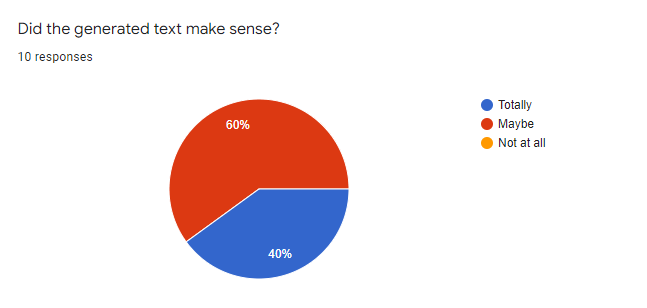
\includegraphics[width=.8\linewidth]{img/feedback0.png}
  \label{fig:feedback0}
\end{figure}
\begin{figure}[ht]
  \centering
  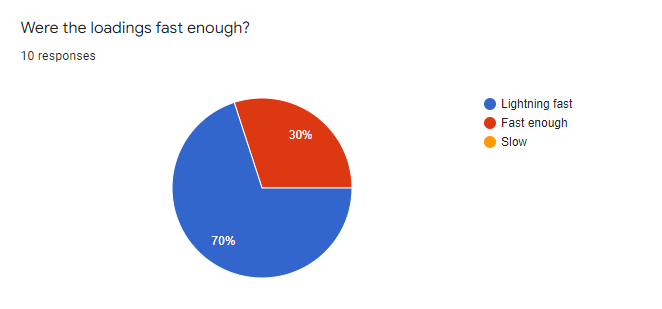
\includegraphics[width=.8\linewidth]{img/feedback1.png}
  \label{fig:feedback1}
\end{figure}
\begin{figure}[ht]
  \centering
  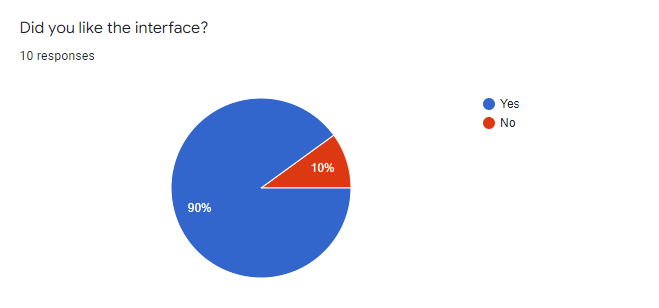
\includegraphics[width=.8\linewidth]{img/feedback2.png}
  \label{fig:feedback2}
\end{figure}
\begin{figure}[ht]
  \centering
  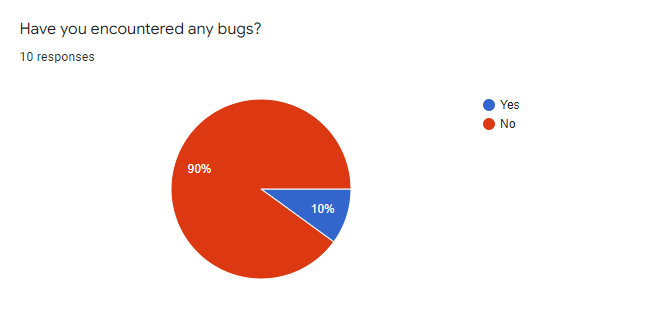
\includegraphics[width=.8\linewidth]{img/feedback3.png}
  \label{fig:feedback3}
\end{figure}
\begin{figure}[ht]
  \centering
  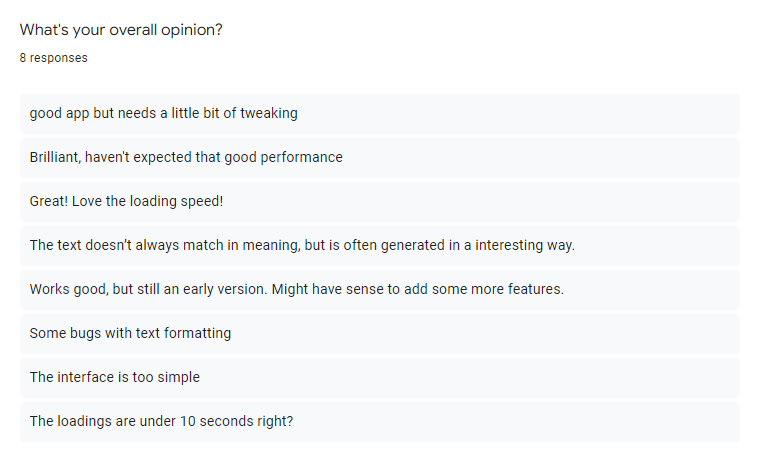
\includegraphics[width=.8\linewidth]{img/feedback4.png}
  \label{fig:feedback4}
\end{figure}

\clearpage

\section*{UML diagram}
\addcontentsline{toc}{section}{UML Diagram}
\label{appendix:uml}

\begin{figure}[ht]
  \centering
  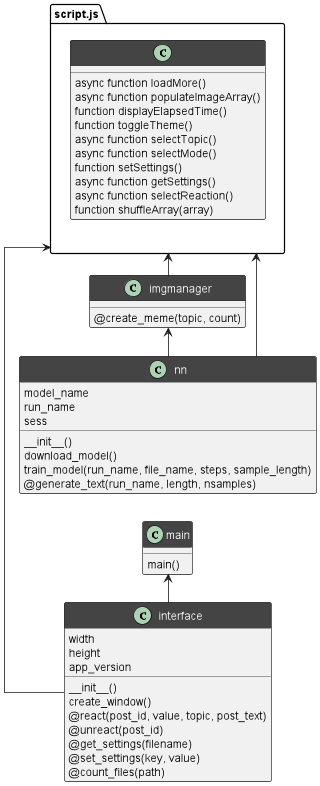
\includegraphics[width=.4\linewidth]{img/uml.png}
  \label{fig:uml}
\end{figure}

\clearpage

\subsection*{UML Diagram Explanation}
\addcontentsline{toc}{subsection}{UML Diagram Explanation}
\label{appendix:uml_explanation}
\paragraph{}
This UML diagram is a representation of the classes and their relationships. Since the program is written in Python, it's
been decided to name the diagram boxes with the names of the files rather than the class names because many of the
methods are static and are not included in the classes and are simply exposed to Eel using the specific decorator -
`@eel.expose'.

The diagram has been created using `PlantUML' which is a tool for creating UML diagrams from source code. It has been
used as a plugin for PyCharm. The final diagram was saved in a PNG file format and is shown in the figure.

The above diagram has 5 classes, 13 non-static methods and 7 static methods. Basically, static methods are methods
that are called from the frontend in the backend and vice versa. Other non-static methods work on their own side and don't cross-talk with
the frontend/backend.

The frontend script file called simply `script.js' is the main JavaScript file and is used exclusively in the frontend.
The main function `loadMore()' is called when the user scrolls to the bottom of the page and makes the program generate
more stories. Every time the user scrolls, also `populateImageArray()' function is called because displaying the stories,
it's necessary to bind them with the images. `displayElapsedTime()' is a function that is called every 60 seconds to display
the time the user has spent in the app. The said time is displayed in the menu. `toggleTheme()' is a function that has
been claimed in the additional feature form. It toggles the theme of the app from light to dark and vice versa. Heavily based
on Bootstrap and the way it works - it toggles the classes of different `DOM' objects on the page since Bootstrap
provide different colours and styles for different themes. `select\_topic()' is used when the user clicks a button with a different
topic than he is on now and it cleans what is currently displayed on the page and displays the stories of the freshly selected topic.
`select\_mode()' is a similar function to `select\_topic()' but it changes the mode of the app from `Classic' to `Meme' and vice versa.
`setSettings()' is used to save the settings of the app in the backend. The previously described functions set the mode, topic and theme in
a specific settings file and then when the app is started these settings are pulled from the file using a function `get\_settings()'
for the app to remember what the user has changed. `selectReaction()' is just a frontend feature to manage the animations
of the like-dislike buttons and maintain the logics behind them (i.e. what can be pressed and what can't). `shuffleArray()'
is a function that shuffles the array of images to make sure that the user doesn't see the same sequence of images every time
the stories are generated.

`imgmanager.py' file contains only one static exposed method `create\_meme(topic, count)'. The method is a more complex piece of code
than the `generate\_text()' function that will follow later, since the later is being called every time the meme is generated.
After it's been generated, the text is split in two parts and appended to the image.

`nn.py' file contains more than just static methods becasue some of the functions written in it are used solely in the
backend. `download\_model()' is used to download and save the desired pretrained model. `train\_model()' is another very used function
in this project because the finetuning process is done through this one. `generate\_text()' function is the one that is
static and is used to generate stories. It takes the run name which can be `Alice', `Cathcer' or `The Iliad', the
length of the desired sample and the number of samples. This is how it works under the hood.

`interface.py' is full of static methods since it mostly operates within the frontend. `react()' and `unreact()' functions
are used to record the reactions for each post in a JSON database, `get\_settings' and `set\_settings' are the backend
implementation of the frontend function with the same names. `count\_files()' is the function that counts files and is used
in the `populateImageArray()' function to determine how many times to iterations to perform.

\end{appendices}

%TC:endignore

\end{document}